% !TeX root = RJwrapper.tex
\title{The mosaic package: helping students to `think with data' using R}
\author{by Randall Pruim, Daniel T Kaplan, Nicholas J Horton}

\maketitle

\abstract{%
The mosaic package provides a simplified and systematic introduction to
the core functionality related to descriptive statistics, visualization,
modeling, and simulation-based inference required in first and second
courses in statistics. This introduction to the package describes some
of the guiding principles behind the design of the package and provides
illustrative examples of several of the most important functions it
implements. These can be combined to help students ``think with data"
using R in their early course work, starting with simple, yet powerful,
declarative commands.
}

\section{Motivation}\label{motivation}

Many have argued that in order to make sense of the increasingly rich
data that is available to them, students need additional facility to
express statistical computations (e.g.,
\cite{NolanTempleLang:2010, Ridgway:2015, HortonBaumerWickham:2015}). To
be able to ``think with data'' (as coined by Diane Lambert of Google),
students need tools for data management, exploratory analysis,
visualization, and modeling. Yet many students enter statistics courses
with little or no computational experience. Our students have
demonstrated that it is feasible to integrate computing into our
curricula early and often, in a way that provides students with success,
confidence, and room to grow.

\section{A guiding principle: Less volume, more
creativity}\label{a-guiding-principle-less-volume-more-creativity}

The \CRANpkg{mosaic} \citep{mosaic} package originated in early attempts
by each of the authors to ease new users into using R, primarily in the
context of undergraduate statistics courses, and, in one case, also in
calculus. One of the guiding principles behind the development of the
\pkg{mosaic} package has been ``Less volume, more creativity''.
Beginners are easily overwhelmed by the scope of R and its many
packages. Often there are multiple ways to accomplish the same task, and
authors of the many packages are not required to follow any particular
style guidelines.

Early on in the development of \pkg{mosaic}, we decided to reduce the
number of code templates that users would need to know to as few as
possible, while still providing them with substantial power to be
creative within the templates provided. A one-page list of commands that
are more than sufficient for a first course, originally presented as
part of a roundtable discussion at the Joint Statistics Meetings
\citep{Pruim:MinimalR:2011} now appears as a vignette in the package,
along with some additional material on the less volume, more creativity
approach.

\section{The formula template}\label{the-formula-template}

To successfully implement a ``less volume, more creativity'' approach,
one must decide which tasks are most important to accomplish. We knew
from the outset that this would include graphical and numerical
summaries of data and various models and inference procedures. Because
of this goal, our most important template makes use of a ``formula
interface'' modeled after \code{lm()} and the plotting functions in
\CRANpkg{lattice} \citep{lattice}.

We typically introduce the formula template in the context of exploring
two variables as

\begin{Schunk}
\begin{Sinput}
goal( y ~ x, data = mydata )    # pseudo-code for the formula template
\end{Sinput}
\end{Schunk}

\noindent
For a plot, \texttt{goal} names the type of plot, \texttt{y} and
\texttt{x} name the variables to be mapped to the vertical and
horizontal axes, and \texttt{mydata} is the data frame in which these
variables are found. This template allows us to create, for example,
scatterplots and side-by-side box plots using \pkg{lattice} functions.
Here we illustrate using the \texttt{Births78} data set from the
\texttt{mosaicData} package, which, as the name suggests, contains data
sets to accompany the \texttt{mosaic} package.

\begin{Schunk}
\begin{Sinput}
require(mosaic)     # instead of library() because students seem to remember it better
xyplot(births ~ date, data = Births78)
\end{Sinput}


\begin{center}\includegraphics[width=.45\textwidth]{pruim-horton-kaplan_files/figure-latex/unnamed-chunk-3-1} \end{center}

\end{Schunk}\begin{Schunk}
\begin{Sinput}
bwplot(births ~ wday, data = Births78) 
bwplot(wday ~ births, data = Births78, pch = "|")
\end{Sinput}


\begin{center}\includegraphics[width=.45\textwidth]{pruim-horton-kaplan_files/figure-latex/unnamed-chunk-4-1} \includegraphics[width=.45\textwidth]{pruim-horton-kaplan_files/figure-latex/unnamed-chunk-4-2} \end{center}

\end{Schunk}

\noindent
The same template can be used to create numerical summaries.

\begin{Schunk}
\begin{Sinput}
mean(births ~ wday, data = Births78)
\end{Sinput}
\begin{Soutput}
##   Sun   Mon  Tues   Wed Thurs   Fri   Sat 
##  7951  9371  9709  9498  9484  9626  8309
\end{Soutput}
\begin{Sinput}
sd(births ~ wday, data = Births78)
\end{Sinput}
\begin{Soutput}
##   Sun   Mon  Tues   Wed Thurs   Fri   Sat 
##   410   608   527   461   551   488   390
\end{Soutput}
\begin{Sinput}
favstats(births ~ wday, data = Births78)
\end{Sinput}
\begin{Soutput}
##    wday  min   Q1 median    Q3   max mean  sd  n missing
## 1   Sun 7135 7691   7936  8196  8711 7951 410 53       0
## 2   Mon 7527 9097   9321  9838 10414 9371 608 52       0
## 3  Tues 8433 9304   9668 10084 10711 9709 527 52       0
## 4   Wed 8606 9196   9362  9880 10703 9498 461 52       0
## 5 Thurs 7915 9171   9397  9958 10499 9484 551 52       0
## 6   Fri 8892 9198   9544 10088 10438 9626 488 52       0
## 7   Sat 7527 8007   8260  8586  9170 8309 390 52       0
\end{Soutput}
\end{Schunk}

\noindent
We introduced the \texttt{tally()} function for counting categorical
variables. We illustrate its use with another data set from
\CRANpkg{mosaicData} \citep{mosaicData}. \texttt{HELPrct} contains data
from the Health Evaluation and Linkage to Primary care study, a clinical
trial for adult inpatients recruited from a detoxification unit. Notice
that in the final example, conditional proportions are calculated.

\begin{Schunk}
\begin{Sinput}
tally(sex ~ substance, data = HELPrct)
\end{Sinput}
\begin{Soutput}
##         substance
## sex      alcohol cocaine heroin
##   female      36      41     30
##   male       141     111     94
\end{Soutput}
\begin{Sinput}
tally(sex ~ substance, data = HELPrct, margins = TRUE)
\end{Sinput}
\begin{Soutput}
##         substance
## sex      alcohol cocaine heroin
##   female      36      41     30
##   male       141     111     94
##   Total      177     152    124
\end{Soutput}
\begin{Sinput}
tally(sex ~ substance, data = HELPrct, margins = TRUE, format = "proportion")
\end{Sinput}
\begin{Soutput}
##         substance
## sex      alcohol cocaine heroin
##   female   0.203   0.270  0.242
##   male     0.797   0.730  0.758
##   Total    1.000   1.000  1.000
\end{Soutput}
\end{Schunk}

Formula interfaces are provided for \texttt{mean()}, \texttt{median()},
\texttt{sd()}, \texttt{var()}, \texttt{cor()}, \texttt{cov()},
\texttt{quantile()}, \texttt{max()}, \texttt{min()}, \texttt{range()},
\texttt{IQR()}, \texttt{iqr()}, \texttt{fivenum()}, \texttt{prod()}, and
\texttt{sum()}. In each case we have been careful not to break behavior
of the underlying functions from \pkg{base} and \pkg{stats}.

The formula template can be extended to handle one variable or more than
two variables, but we recommend introducing it in the context of
two-variable plots and summaries. This is for several reasons: (1)
two-variable plots and numerical summaries are more ``impressive'' and
less likely to be something students can as readily do with tools they
already know, (2) working with more than one variable from the start
(correctly) suggests that the most interesting parts of statistics
involve more than one variable \citep{Wild:RSS:2011}, and (3) the
formula syntax for a single variable makes more sense in the context of
two-sided formulas that it does in isolation.

Once the two-variable summaries are understood, we can add a third or
fourth variable with

\begin{Schunk}
\begin{Sinput}
goal( y ~ x | z, groups = mygroups, data=mydata )    # pseudo-code
\end{Sinput}
\end{Schunk}

\noindent
When plotting, \texttt{z} is used to create plots with subpanels (or
facets) and \texttt{groups} indicates overlaid layers.

\begin{Schunk}
\begin{Sinput}
xyplot(births ~ date, groups = wday, data = Births78, type = "l")
densityplot( ~ births, groups = wday, data = Births78, auto.key=list(columns=3))
\end{Sinput}


\begin{center}\includegraphics[width=.45\textwidth]{pruim-horton-kaplan_files/figure-latex/unnamed-chunk-8-1} \includegraphics[width=.45\textwidth]{pruim-horton-kaplan_files/figure-latex/unnamed-chunk-8-2} \end{center}

\end{Schunk}\begin{Schunk}
\begin{Sinput}
densityplot( ~ age | sex, groups = substance, data = HELPrct)
bwplot( age ~ substance | sex, data = HELPrct)
\end{Sinput}


\begin{center}\includegraphics[width=.45\textwidth]{pruim-horton-kaplan_files/figure-latex/unnamed-chunk-9-1} \includegraphics[width=.45\textwidth]{pruim-horton-kaplan_files/figure-latex/unnamed-chunk-9-2} \end{center}

\end{Schunk}

For numerical summaries the condition \texttt{z} and \texttt{groups}
play essentially the same role, so each of the following produces an
equivalent result.

\begin{Schunk}
\begin{Sinput}
mean( age ~ sex, data = HELPrct)
\end{Sinput}
\end{Schunk}\begin{Schunk}
\begin{Sinput}
mean( ~ age | sex, data = HELPrct)
\end{Sinput}
\end{Schunk}\begin{Schunk}
\begin{Sinput}
mean( ~ age, groups = sex, data = HELPrct)
\end{Sinput}
\begin{Soutput}
## female   male 
##   36.3   35.5
\end{Soutput}
\end{Schunk}

\noindent
This allows us to compute numerical summaries by replacing the name of
the plot with the name of the desired summary.

The one-variable template can be obtained by removing the left-hand side
from the formula in a two-variable template.

\begin{Schunk}
\begin{Sinput}
goal( ~ x, data=mydata )               # psuedo-code
\end{Sinput}
\end{Schunk}

\noindent
In the context of plotting, this makes sense since we are providing the
data for the \(x\)-axis and allowing R to compute values for the
\(y\)-axis:

\begin{Schunk}
\begin{Sinput}
histogram( ~ age, data = HELPrct)
\end{Sinput}


\begin{center}\includegraphics[width=.45\textwidth]{pruim-horton-kaplan_files/figure-latex/unnamed-chunk-14-1} \end{center}

\end{Schunk}

\noindent
Numerical summaries fit this pattern by analogy (and because R formulas
are required to have a right hand side).

\begin{Schunk}
\begin{Sinput}
mean( ~ age, data = HELPrct)
\end{Sinput}
\begin{Soutput}
## [1] 35.7
\end{Soutput}
\end{Schunk}

As students become familiar with the formula interface, all three forms
can be brought together into a single template:

\begin{Schunk}
\begin{Sinput}
goal( formula, data=mydata, ... )      # psuedo-code
\end{Sinput}
\end{Schunk}

\noindent
The formula template allows students to think about relationships
between and among two or more variables and to test conjectures using
graphical and numerical summaries. Having learned the formula interface
to graphical and numerical summaries early on, new users are well
prepared for modeling with \code{lm()}, \code{glm()}, and various
``test'' functions such as \texttt{t.test()} when the time comes. More
importantly, they begin early to train their minds to ask questions of
the form ``How does this depend on that (and some other things)?''.

By emphasizing the formula template, each of the following commands can
be viewed as instances of a common template, rather than as separate
things to learn.

\begin{Schunk}
\begin{Sinput}
bwplot(age ~ sex, data=HELPrct)
  mean(age ~ sex, data=HELPrct)
    sd(age ~ sex, data=HELPrct)
    lm(age ~ sex, data=HELPrct)
t.test(age ~ sex, data=HELPrct) 
\end{Sinput}
\end{Schunk}

\noindent
Similarly, by adding additional formula interfaces to \texttt{t.test()},
\texttt{binom.test()}, and \texttt{prop.test()}, and adding some
additional plot types, for one-variable situations we have

\begin{Schunk}
\begin{Sinput}
       mean( ~ age, data=HELPrct)
         sd( ~ age, data=HELPrct)
   favstats( ~ age, data=HELPrct)
  histogram( ~ age, data=HELPrct)
    dotPlot( ~ age, data=HELPrct)   # dot plots
freqpolygon( ~ age, data=HELPrct)   # frequency polygon
    ashplot( ~ age, data=HELPrct)   # average shifted histogram
     t.test( ~ age, data=HELPrct)   # formula interface added in mosaic
 binom.test( ~ sex, data=HELPrct)   # formula interface added in mosaic
  prop.test( ~ sex, data=HELPrct)   # formula interface added in mosaic
\end{Sinput}
\end{Schunk}

\noindent
Adding covariates to one- or two- variable graphical or numerical
summaries fits readily into the template as well.

\begin{Schunk}
\begin{Sinput}
     mean( ~ age | sex, data=HELPrct)
       sd( ~ age | sex, data=HELPrct)
histogram( ~ age | sex, data=HELPrct)
   t.test( ~ age | sex, data=HELPrct)
\end{Sinput}
\end{Schunk}

While creating the correct formula can produce some challenges for new
users, clearly explaining the roles of each component for plotting, for
numerical summaries, and for model fitting helps demystify the
situation. Instructors have had students create and interpret bivariate
and trivariate graphical displays on the first day of class
\citep{Wang:USCOTS:2015}. We have also found that explicit, early,
low-stakes assessment of student mastery of the formula interface
greatly improves student performance. A first quiz consisting of a
single item (What is the formula template?) followed by one or two
simple pencil-and-paper quizzes asking students to write the commands to
recreate a handful of numerical and graphical summaries suffices.

\subsection{Handling missing data}\label{handling-missing-data}

When there are missing values, the numerical summary functions in
\pkg{base} and \pkg{stats} return results that may surprise and mystify
new users.

\begin{Schunk}
\begin{Sinput}
mean( ~ dayslink, data = HELPmiss)
\end{Sinput}
\begin{Soutput}
## [1] NA
\end{Soutput}
\end{Schunk}

\noindent
While there are workarounds using options to functions to drop values
that are missing before performing the computation, these may be
intimidating to new users.

\begin{Schunk}
\begin{Sinput}
mean( ~ dayslink, data = HELPmiss, na.rm = TRUE)
\end{Sinput}
\begin{Soutput}
## [1] 257
\end{Soutput}
\end{Schunk}

We offer two other solutions to this situation. Our favorite is the
\texttt{favstats()} function which computes a set of useful numerical
summaries on the non-missing values and also reports the number of
missing values.

\begin{Schunk}
\begin{Sinput}
favstats( ~ dayslink, data = HELPmiss)
\end{Sinput}
\begin{Soutput}
##  min Q1 median  Q3 max mean  sd   n missing
##    2 75    363 365 456  257 151 447      23
\end{Soutput}
\end{Schunk}

The second solution is to change the default behavior of \texttt{na.rm}
using \texttt{options()}. This will, of course, only affect the
\pkg{mosaic} versions of these functions.

\begin{Schunk}
\begin{Sinput}
options(na.rm = TRUE)
mean(~ dayslink, data = HELPmiss)
\end{Sinput}
\begin{Soutput}
## [1] 257
\end{Soutput}
\begin{Sinput}
with(HELPmiss, base::mean(dayslink))
\end{Sinput}
\begin{Soutput}
## [1] NA
\end{Soutput}
\end{Schunk}

\noindent
Users also have the option of changing the default for \texttt{na.rm}
back if they like.

\begin{Schunk}
\begin{Sinput}
options(na.rm = NULL)
mean(~ dayslink, data = HELPmiss)
\end{Sinput}
\begin{Soutput}
## [1] NA
\end{Soutput}
\end{Schunk}

\subsection{Inspecting a data frame}\label{inspecting-a-data-frame}

Summaries of all variables in a data frame can be obtained using
\texttt{inspect()}. For quantitative variables, the results of
\texttt{favstats()} are displayed. Other summaries are provided for
categorical and time variables.

\begin{Schunk}
\begin{Sinput}
inspect(Births78)
\end{Sinput}
\begin{Soutput}
## 
## categorical variables:  
##   name   class levels   n missing                                  distribution
## 1 wday ordered      7 365       0 Sun (14.5%), Mon (14.2%), Tues (14.2%) ...   
## 
## quantitative variables:  
##        name   class  min   Q1 median   Q3   max mean  sd   n missing
## 1    births integer 7135 8554   9218 9705 10711 9132 818 365       0
## 2 dayofyear integer    1   92    183  274   365  183 106 365       0
## 
## time variables:  
##   name   class      first       last min_diff max_diff   n missing
## 1 date POSIXct 1978-01-01 1978-12-31        1        1 365       0
\end{Soutput}
\end{Schunk}

\subsection{Creating and using
functions}\label{creating-and-using-functions}

Especially in calculus, but also when modeling in statistics, it is
useful to create functions defined by algebraic formulas. With
\texttt{makeFun()} we can construct such functions using a formula
interface and use \texttt{plotFun()} to plot them.

\begin{Schunk}
\begin{Sinput}
f <- makeFun(A + B * log(x) ~ x, A = 1, B = 1)
f
\end{Sinput}
\begin{Soutput}
## function (x, A = 1, B = 1) 
## A + B * log(x)
\end{Soutput}
\begin{Sinput}
f(2)
\end{Sinput}
\begin{Soutput}
## [1] 1.69
\end{Soutput}
\begin{Sinput}
plotFun(f(x) ~ x, xlim = c(0,3))
\end{Sinput}


\begin{center}\includegraphics[width=.45\textwidth]{pruim-horton-kaplan_files/figure-latex/unnamed-chunk-26-1} \end{center}

\end{Schunk}

More interestingly for statistics, we can use \texttt{makeFun()} to
create functions from model objects created by \texttt{lm()} and
\texttt{glm()}.

\begin{Schunk}
\begin{Sinput}
cars.mod1 <- lm(dist ~ speed, data = cars)
cars.mod2 <- lm(dist ~ poly(speed,2), data = cars)
dist1 <- makeFun(cars.mod1)
dist2 <- makeFun(cars.mod2)
dist2(speed = 15)
\end{Sinput}
\begin{Soutput}
##    1 
## 38.7
\end{Soutput}
\begin{Sinput}
dist2(speed = 15, interval = "confidence")
\end{Sinput}
\begin{Soutput}
##    fit lwr  upr
## 1 38.7  33 44.3
\end{Soutput}
\begin{Sinput}
xyplot(dist ~ speed, data = cars, alpha = 0.4)
plotFun(dist1(s) ~ s, add = TRUE, col = 2, lwd = 2)
plotFun(dist2(s) ~ s, add = TRUE, col = 3, lwd = 2)
\end{Sinput}


\begin{center}\includegraphics[width=.45\textwidth]{pruim-horton-kaplan_files/figure-latex/unnamed-chunk-27-1} \end{center}

\end{Schunk}

\noindent
For logistic regression, when the response is coded as a factor, we need
to adjust things slightly when plotting because the model function
returns values between 0 and 1, but 2-level factors are coded as 1 and
2.

\begin{Schunk}
\begin{Sinput}
Feet.mod <- glm(sex ~ width, data = KidsFeet, family = binomial)
s <- makeFun(Feet.mod)
s(width = 8.5)
\end{Sinput}
\begin{Soutput}
##     1 
## 0.704
\end{Soutput}
\begin{Sinput}
xyplot(sex ~ width, data = KidsFeet, jitter.y = TRUE)
plotFun(1 + s(w) ~ w, add = TRUE)
\end{Sinput}


\begin{center}\includegraphics[width=.45\textwidth]{pruim-horton-kaplan_files/figure-latex/unnamed-chunk-28-1} \end{center}

\end{Schunk}

This wrapper around \texttt{predict()} is easier for beginners to use
because (a) it returns a function to which inputs can be supplied
without creating a data frame, (b) the resulting function returns values
on the response scale by default, and (c) it back transforms a few
common transformations of the response variable, including
\texttt{log()} and \texttt{sqrt()} (and allows the user to provide a
custom value to the \texttt{transform} argument to handle other cases).

\begin{Schunk}
\begin{Sinput}
mtcars.mod <- lm(log(mpg) ~ log(wt) + factor(cyl), data = mtcars)
mileage <- makeFun(mtcars.mod)
xyplot(mpg ~ wt, data = mtcars, groups = cyl)
plotFun( mileage(w, cyl=4) ~ w, add = TRUE, col = 1)
plotFun( mileage(w, cyl=6) ~ w, add = TRUE, col = 2)
plotFun( mileage(w, cyl=8) ~ w, add = TRUE, col = 3)
\end{Sinput}


\begin{center}\includegraphics[width=.45\textwidth]{pruim-horton-kaplan_files/figure-latex/unnamed-chunk-29-1} \end{center}

\end{Schunk}

For many simple models, creating a plot can be even simpler using
\texttt{plotModel()}, which also eliminates the need to manually adjust
logistic regression plots when the response is a factor.

\begin{Schunk}
\begin{Sinput}
plotModel(cars.mod2)
plotModel(Feet.mod, jitter.y = TRUE)
\end{Sinput}


\begin{center}\includegraphics[width=.45\textwidth]{pruim-horton-kaplan_files/figure-latex/unnamed-chunk-30-1} \includegraphics[width=.45\textwidth]{pruim-horton-kaplan_files/figure-latex/unnamed-chunk-30-2} \end{center}

\end{Schunk}

\noindent
The \texttt{plotModel()} function can also simplify visualization of
more complex models.

\begin{Schunk}
\begin{Sinput}
mtcars.mod2 <- lm(mpg ~ log(wt) + factor(cyl) + factor(am), data = mtcars)
plotModel(mtcars.mod2, mpg ~ wt | factor(am))
\end{Sinput}


\begin{center}\includegraphics[width=.45\textwidth]{pruim-horton-kaplan_files/figure-latex/unnamed-chunk-31-1} \end{center}

\end{Schunk}

\section{Randomization and
Resampling}\label{randomization-and-resampling}

Resampling approaches have become increasingly important in statistical
education \citep{Tintle:TAS:2015, Hesterberg:2015}. The \pkg{mosaic}
package provides simplified functionality to support teaching inference
based on randomization tests and bootstrap methods. Our goal was to
focus attention on the important parts of these techniques (e.g., where
randomness enters in and how to use the resulting distribution) while
hiding some of the technical details involved in creating loops and
accumulating values.

\subsection{A first example}\label{a-first-example}

As a first example, we often introduce the story of the lady tasting
tea. (See \cite{Salsburg:2002} for the details of this famous story.)
But here we will test a coin to see whether it is a ``fair coin''.
Suppose we flip the coin 20 times and observe only 6 heads, how
suspicious should we be that the coin is not fair? The statistical
punchline for either the lady tasting tea or testing a coin is that we
want to compute the p-value for a binomial test via simulations rather
than using formulas for the binomial distribution or normal
approximations. But we want to do this on the first day of class, and
without using any of the jargon of the preceding sentence.

Because students do not know about sampling distributions or random
variables yet, but do understand the idea of a coin toss, we have
provided \texttt{rflip()} to simulate tossing a coin one or several
times:

\begin{Schunk}
\begin{Sinput}
rflip()
\end{Sinput}
\begin{Soutput}
## 
## Flipping 1 coin [ Prob(Heads) = 0.5 ] ...
## 
## H
## 
## Number of Heads: 1 [Proportion Heads: 1]
\end{Soutput}
\begin{Sinput}
rflip(20)
\end{Sinput}
\begin{Soutput}
## 
## Flipping 20 coins [ Prob(Heads) = 0.5 ] ...
## 
## T H T H H H H H H H T T T T H H T H H T
## 
## Number of Heads: 12 [Proportion Heads: 0.6]
\end{Soutput}
\end{Schunk}

To test a null hypothesis of a fair coin, we need to simulate flipping
20 coins many times, recording for each simulation the number of heads
that were observed. The \texttt{do()} function allows us to do just that
using the following template

\begin{Schunk}
\begin{Sinput}
do(n) * {stuff to do}             # pseudo-code
\end{Sinput}
\end{Schunk}

\noindent
where \texttt{\{stuff\ to\ do\}} is typically a single R command, but
may be something more complicated. For example, we can flip 20 coins
three times as follows.

\begin{Schunk}
\begin{Sinput}
do(3) * rflip(20)
\end{Sinput}
\begin{Soutput}
##    n heads tails prop
## 1 20    11     9 0.55
## 2 20     9    11 0.45
## 3 20     9    11 0.45
\end{Soutput}
\end{Schunk}

\noindent
Notice that \texttt{do()} (technically \texttt{cull\_for\_do()}) has
been clever about what information is stored for each group of 20 coin
tosses. It is now a simple matter to do this many more times and use
numerical or graphical summaries to investigate how unusual it is to get
so few heads if the coin is indeed a fair coin.

\begin{Schunk}
\begin{Sinput}
Sims <- do (1000) * rflip(20)
histogram( ~ heads, data = Sims, width = 1, groups = heads <= 6)
tally ( ~(heads <= 6), data = Sims)
\end{Sinput}
\begin{Soutput}
## 
##  TRUE FALSE 
##    58   942
\end{Soutput}


\begin{center}\includegraphics[width=.45\textwidth]{pruim-horton-kaplan_files/figure-latex/unnamed-chunk-35-1} \end{center}

\end{Schunk}

\noindent
(If you are familiar with \pkg{lattice}, you will notice that the
\pkg{mosaic} package also adds some additional arguments to the
\texttt{histogram()} function.)

\subsection{sample(), resample(), and
shuffle()}\label{sample-resample-and-shuffle}

To facilitate randomization and bootstrapping, \pkg{mosaic} extends
\texttt{sample()} to operate on data frames. The \texttt{shuffle()}
function is an alternative name for \texttt{sample()}, and
\texttt{resample()} is \texttt{sample()} with \texttt{replace\ =\ TRUE}.
With these in hand, all of the tests and confidence intervals seen in a
traditional first course in statistics can be performed using a common
outline:

\begin{enumerate}
\def\labelenumi{\arabic{enumi}.}
\tightlist
\item
  Do it to your data
\item
  Do it to a randomized version of your data
\item
  Do it to lots of randomized versions of your data.
\end{enumerate}

For example, we can use randomization in place of the two-sample t test
to obtain an empirical p-value.

\begin{Schunk}
\begin{Sinput}
D <- diffmean(age ~ sex, data = HELPrct); D 
\end{Sinput}
\begin{Soutput}
## diffmean 
##   -0.784
\end{Soutput}
\begin{Sinput}
do(1) * diffmean(age ~ shuffle(sex), data = HELPrct)
\end{Sinput}
\begin{Soutput}
##   diffmean
## 1   -0.601
\end{Soutput}
\begin{Sinput}
Null.dist <- do(5000) * diffmean(age ~ shuffle(sex), data = HELPrct)
histogram( ~ diffmean, data = Null.dist, v = D)
prop( ~ (diffmean < D), data = Null.dist, format = "prop")
\end{Sinput}
\begin{Soutput}
##  TRUE 
## 0.176
\end{Soutput}


\begin{center}\includegraphics[width=.45\textwidth]{pruim-horton-kaplan_files/figure-latex/do-diff-mean-1} \end{center}

\end{Schunk}

\begin{Schunk}
\begin{Sinput}
pval(t.test(age ~ sex, data = HELPrct, alternative = "greater"))
\end{Sinput}
\begin{Soutput}
## p.value 
##   0.177
\end{Soutput}
\end{Schunk}

The example above introduces three additional \pkg{mosaic} functions.
The \texttt{prop()} function computes the proportion of logical vector
that is (by default) \texttt{TRUE} or of a factor that is (by default)
the first label; \texttt{diffmean()} is similar to
\texttt{diff(mean())}, but labels the result differently
(\texttt{diffprop()} works similarly for differences in proportions);
and \texttt{pval()} extracts the p-value from an object of class
\texttt{"htest"}.

It should be noted that although this is typically not done in
simulation-based introductory statistics texts, one might prefer to
calculate p-values by including the observed data in the randomization
distribution. This avoids an empirical p-value of 0 and guarantees that
the actual type I error rate will not exceed the nominal type I error
rate.

\begin{Schunk}
\begin{Sinput}
count( ~ (diffmean < D), data = Null.dist)
\end{Sinput}
\begin{Soutput}
##  TRUE 
## 0.176
\end{Soutput}
\begin{Sinput}
(1 + count( ~ (diffmean < D), data = Null.dist)) / (1 + nrow(Null.dist))  # p-value
\end{Sinput}
\begin{Soutput}
##     TRUE 
## 0.000235
\end{Soutput}
\end{Schunk}

If we are interested in a confidence interval for the difference in
group means, we can use \texttt{resample()} and \texttt{do()} to
generate a bootstrap distribution in one of two ways.

\begin{Schunk}
\begin{Sinput}
Boot.dist1 <- do(1000) * diffmean(age ~ sex, data = resample(HELPrct))
Boot.dist2 <- do(1000) * diffmean(age ~ sex, data = resample(HELPrct, groups = sex))
\end{Sinput}
\end{Schunk}

\noindent
In the second example, the resampling happens within the sex groups so
that the marginal counts for each sex remain fixed. This can be
especially important if one of the groups is small, because otherwise
some resamples might not include any observations of that group.

\begin{Schunk}
\begin{Sinput}
favstats(age ~ sex, data = HELPrct)
\end{Sinput}
\begin{Soutput}
##      sex min Q1 median   Q3 max mean   sd   n missing
## 1 female  21 31     35 40.5  58 36.3 7.58 107       0
## 2   male  19 30     35 40.0  60 35.5 7.75 346       0
\end{Soutput}
\begin{Sinput}
favstats(age ~ sex, data = resample(HELPrct))
\end{Sinput}
\begin{Soutput}
##      sex min Q1 median Q3 max mean   sd   n missing
## 1 female  21 30     34 39  58 35.3 7.80  98       0
## 2   male  19 30     35 39  58 35.3 7.59 355       0
\end{Soutput}
\begin{Sinput}
favstats(age ~ sex, data = resample(HELPrct, groups = sex))
\end{Sinput}
\begin{Soutput}
##      sex min Q1 median Q3 max mean   sd   n missing
## 1 female  21 31     37 40  58 37.2 7.93 107       0
## 2   male  19 30     35 41  60 35.7 7.95 346       0
\end{Soutput}
\end{Schunk}

Using either bootstrap distribution, two simple confidence intervals can
be computed. We typically introduce percentile confidence intervals
first. A percentile confidence interval is calculated by determining the
range of a central portion of the bootstrap distribution, which can be
automated using \texttt{cdata()}. Visually inspecting the bootstrap
distribution for skew and bias is an important step to make sure the
percentile interval is not being applied in a situation where it may
perform poorly.

\begin{Schunk}
\begin{Sinput}
histogram( ~ diffmean, data = Boot.dist2, v = D)
qqmath( ~ diffmean, data = Boot.dist2)
cdata( ~ diffmean, p = 0.95, data = Boot.dist2)
\end{Sinput}
\begin{Soutput}
##       low        hi central.p 
##    -2.473     0.913     0.950
\end{Soutput}


\begin{center}\includegraphics[width=.45\textwidth]{pruim-horton-kaplan_files/figure-latex/unnamed-chunk-42-1} \includegraphics[width=.45\textwidth]{pruim-horton-kaplan_files/figure-latex/unnamed-chunk-42-2} \end{center}

\end{Schunk}

Alternatively, we can compute a confidence interval based on a bootstrap
estimate of the standard error.

\begin{Schunk}
\begin{Sinput}
SE <- sd( ~ diffmean, data = Boot.dist2); SE
\end{Sinput}
\begin{Soutput}
## [1] 0.867
\end{Soutput}
\begin{Sinput}
D + c(-1,1) * 2 * SE
\end{Sinput}
\begin{Soutput}
## [1] -2.519  0.951
\end{Soutput}
\end{Schunk}

\noindent
The primary pedagogical value of the bootstrap standard error approach
is its close connection to the standard formula-based confidence
interval methods. How to replace the constant 2 with an appropriate
value to create more accurate intervals or to allow for different
confidence levels is a matter of some subtlety \citep{Hesterberg:2015}.
The simplest method is to use quantiles of a normal distribution, but
this will undercover. Replacing the normal distribution with an
appropriate t-distribution will widen intervals and can improve
coverage, but the t-distribution is only correct in a few cases -- such
as when estimating the mean of a normal population -- and can perform
badly when the population is skewed. See the Discussion Section for more
on this.

Calculating simple confidence intervals can be further automated using
an extension to \texttt{confint()}.

\begin{Schunk}
\begin{Sinput}
confint(Boot.dist2, method = c("percentile", "stderr"))
\end{Sinput}
\begin{Soutput}
##       name lower upper level     method estimate margin.of.error  df
## 1 diffmean -2.47 0.913  0.95 percentile   -0.784              NA  NA
## 2 diffmean -2.48 0.933  0.95     stderr   -0.784             1.7 452
\end{Soutput}
\end{Schunk}

\section{Extracting information}\label{extracting-information}

Modeled on functions like \code{resid()}, a number of additional
functions have been added to \pkg{mosaic} to facilitate extracting
information from more complicated objects. Some examples include

\begin{Schunk}
\begin{Sinput}
confint(t.test( ~ age, data = HELPrct))    # works for any "htest" object
\end{Sinput}
\begin{Soutput}
##   mean of x lower upper level
## 1      35.7  34.9  36.4  0.95
\end{Soutput}
\begin{Sinput}
pval(t.test(age ~ sex, data = HELPrct))    # works for any "htest" object
\end{Sinput}
\begin{Soutput}
## p.value 
##   0.354
\end{Soutput}
\begin{Sinput}
stat(t.test(age ~ sex, data = HELPrct))    # works for any "htest" object
\end{Sinput}
\begin{Soutput}
##    t 
## 0.93
\end{Soutput}
\begin{Sinput}
rsquared(lm(age ~ sex, data=HELPrct))
\end{Sinput}
\begin{Soutput}
## [1] 0.00187
\end{Soutput}
\end{Schunk}

\section{Some additional visualization
tools}\label{some-additional-visualization-tools}

\subsection{Additional high-level lattice
plots}\label{additional-high-level-lattice-plots}

The \pkg{mosaic} package provides several new high-level \pkg{lattice}
plots, including \texttt{bargraph()}, \texttt{dotPlot()},
\texttt{freqpolygon()}, \texttt{ashplot()}, \texttt{xqqmath()}, and
\texttt{plotPoints()}.

\begin{Schunk}
\begin{Sinput}
bargraph( ~ substance, data = HELPrct, main = "bargraph")
dotPlot( ~ age, data = HELPrct, width = 1, main = "dotPlot")
\end{Sinput}


\begin{center}\includegraphics[width=.45\textwidth]{pruim-horton-kaplan_files/figure-latex/unnamed-chunk-45-1} \includegraphics[width=.45\textwidth]{pruim-horton-kaplan_files/figure-latex/unnamed-chunk-45-2} \end{center}

\end{Schunk}\begin{Schunk}
\begin{Sinput}
freqpolygon( ~ age, data = HELPrct, width = 2, main = "freqpolygon")
ashplot( ~ age, data = HELPrct, width = 2, main = "ashplot")
\end{Sinput}


\begin{center}\includegraphics[width=.45\textwidth]{pruim-horton-kaplan_files/figure-latex/unnamed-chunk-46-1} \includegraphics[width=.45\textwidth]{pruim-horton-kaplan_files/figure-latex/unnamed-chunk-46-2} \end{center}

\end{Schunk}\begin{Schunk}
\begin{Sinput}
xqqmath( ~ age, data = HELPrct, main = "xqqmath")
plotPoints(length ~ width, data = KidsFeet, main = "plotPoints")
\end{Sinput}


\begin{center}\includegraphics[width=.45\textwidth]{pruim-horton-kaplan_files/figure-latex/unnamed-chunk-47-1} \includegraphics[width=.45\textwidth]{pruim-horton-kaplan_files/figure-latex/unnamed-chunk-47-2} \end{center}

\end{Schunk}

\subsection{Visualizing distributions of random
variables}\label{visualizing-distributions-of-random-variables}

A number of functions make it simple to visualize random variables.
\texttt{plotDist()} creates displays for any distribution for which
standard d-, p-, and q- functions exist.

\begin{Schunk}
\begin{Sinput}
plotDist("norm", mean = 100, sd = 10)
plotDist("binom", size = 100, prob = 0.3)
\end{Sinput}


\begin{center}\includegraphics[width=.45\textwidth]{pruim-horton-kaplan_files/figure-latex/unnamed-chunk-48-1} \includegraphics[width=.45\textwidth]{pruim-horton-kaplan_files/figure-latex/unnamed-chunk-48-2} \end{center}

\end{Schunk}

\noindent
Tail probabilities can be highlighted using the \texttt{groups}
argument.

\begin{Schunk}
\begin{Sinput}
plotDist("chisq", df = 4, groups = x > 9)
plotDist("chisq", df = 4, groups = x > 9, type = "h")
\end{Sinput}


\begin{center}\includegraphics[width=.45\textwidth]{pruim-horton-kaplan_files/figure-latex/unnamed-chunk-49-1} \includegraphics[width=.45\textwidth]{pruim-horton-kaplan_files/figure-latex/unnamed-chunk-49-2} \end{center}

\end{Schunk}

\noindent
Using the \texttt{kind} argument, we can obtain other types of plots,
including cdfs and probability histograms.

\begin{Schunk}
\begin{Sinput}
plotDist("norm", mean = 100, sd = 10, kind = "cdf")
plotDist("binom", size = 100, prob = 0.3, kind = "histogram")
\end{Sinput}


\begin{center}\includegraphics[width=.45\textwidth]{pruim-horton-kaplan_files/figure-latex/unnamed-chunk-50-1} \includegraphics[width=.45\textwidth]{pruim-horton-kaplan_files/figure-latex/unnamed-chunk-50-2} \end{center}

\end{Schunk}

For several distributions, we provide augmented versions of the
distribution and quantile functions that assist students in
understanding what values are returned by functions like
\texttt{pnorm()} and \texttt{qnorm()}.

\begin{Schunk}
\begin{Sinput}
xpnorm(-2:2)
\end{Sinput}
\begin{Soutput}
## 
## If X ~ N(0,1), then 
## 
##  P(X <= -2) = P(Z <= -2) = 0.0228
##      P(X <= -1) = P(Z <= -1) = 0.1587
##      P(X <= 0) = P(Z <= 0) = 0.5
##      P(X <= 1) = P(Z <= 1) = 0.8413
##      P(X <= 2) = P(Z <= 2) = 0.9772
##  P(X >  -2) = P(Z >  -2) = 0.9772
##      P(X >  -1) = P(Z >  -1) = 0.8413
##      P(X >  0) = P(Z >  0) = 0.5
##      P(X >  1) = P(Z >  1) = 0.1587
##      P(X >  2) = P(Z >  2) = 0.0228
\end{Soutput}
\begin{Soutput}
## [1] 0.0228 0.1587 0.5000 0.8413 0.9772
\end{Soutput}
\begin{Sinput}
xqt(0.975, df = 20)
\end{Sinput}
\begin{Soutput}
## [1] 2.09
\end{Soutput}


\begin{center}\includegraphics[width=.45\textwidth]{pruim-horton-kaplan_files/figure-latex/unnamed-chunk-51-1} \includegraphics[width=.45\textwidth]{pruim-horton-kaplan_files/figure-latex/unnamed-chunk-51-2} \end{center}

\end{Schunk}

\subsection{mplot()}\label{mplot}

The \texttt{mplot()} function has two primary use cases: creating
diagnostic plots for lm and glm objects, and interactively creating data
visualizations using the variables in a data frame. Given a model object
as its first argument, \texttt{mplot()} provides similar diagnostic
plots to those produced via \texttt{plot()} but with two primary
differences: the user may select to use either \pkg{lattice} or
\CRANpkg{ggplot2} \citep{ggplot2} graphics instead of base graphics, and
an additional plot type is provided to visualize the confidence
intervals for the coefficients of the model.

\begin{Schunk}
\begin{Sinput}
mod <- lm(length ~ width * sex, data = KidsFeet)
mplot(mod, system = "lattice", which = 1:4)
\end{Sinput}


\begin{center}\includegraphics[width=.45\textwidth]{pruim-horton-kaplan_files/figure-latex/unnamed-chunk-52-1} \includegraphics[width=.45\textwidth]{pruim-horton-kaplan_files/figure-latex/unnamed-chunk-52-2} \includegraphics[width=.45\textwidth]{pruim-horton-kaplan_files/figure-latex/unnamed-chunk-52-3} \includegraphics[width=.45\textwidth]{pruim-horton-kaplan_files/figure-latex/unnamed-chunk-52-4} \end{center}

\end{Schunk}\begin{Schunk}
\begin{Sinput}
mplot(mod, system = "ggplot2", which = 4:7)
\end{Sinput}


\begin{center}\includegraphics[width=.45\textwidth]{pruim-horton-kaplan_files/figure-latex/unnamed-chunk-53-1} \includegraphics[width=.45\textwidth]{pruim-horton-kaplan_files/figure-latex/unnamed-chunk-53-2} \includegraphics[width=.45\textwidth]{pruim-horton-kaplan_files/figure-latex/unnamed-chunk-53-3} \includegraphics[width=.45\textwidth]{pruim-horton-kaplan_files/figure-latex/unnamed-chunk-53-4} \end{center}

\end{Schunk}

We can also use \texttt{mplot()} to visually represent the results of
\texttt{TukeyHSD()}, which we can apply directly to objects produced by
\texttt{lm()}.

\begin{Schunk}
\begin{Sinput}
mplot(TukeyHSD(lm(births ~ wday, data = Births78)), order = "pval")
mplot(TukeyHSD(lm(births ~ wday, data = Births78)), order = "pval", system = "ggplot2") 
\end{Sinput}


\begin{center}\includegraphics[width=.45\textwidth]{pruim-horton-kaplan_files/figure-latex/unnamed-chunk-54-1} \includegraphics[width=.45\textwidth]{pruim-horton-kaplan_files/figure-latex/unnamed-chunk-54-2} \end{center}

\end{Schunk}

\noindent
Again, there are options to create either \pkg{lattice} or \pkg{ggplot2}
plots, and the resulting plots are formatted in a way that makes them
usable in a wider range of scenarios than are those produced using
\texttt{plot()}.

A second use for \texttt{mplot()} is to create \pkg{lattice} and
\pkg{ggplot2} plots interactively within RStudio. Issuing the following
command in RStudio will bring up a plot that can be modified by making
choices interactively.

\begin{Schunk}
\begin{Sinput}
mplot(HELPrct)
\end{Sinput}
\end{Schunk}

\begin{figure}
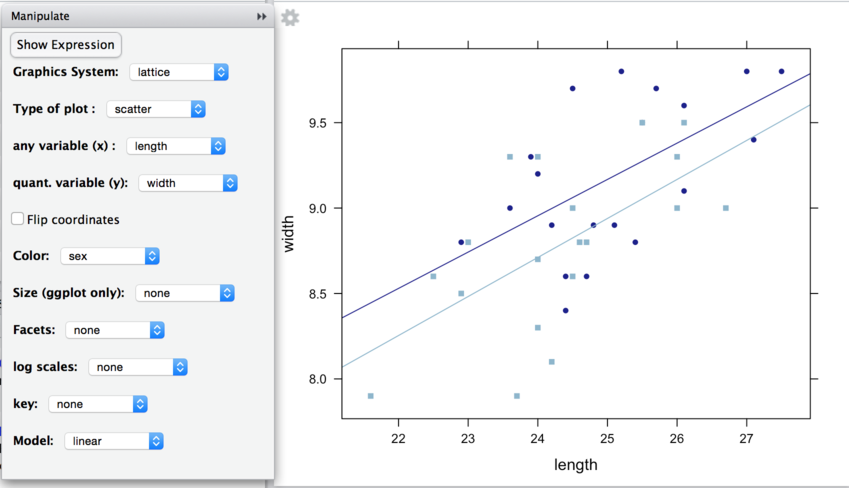
\includegraphics{half-mplot.png}
\caption{In RStudio, \texttt{mplot()} can be used to interactively generate 
plots using variables in a data frame.}
\label{fig:mplot}
\end{figure}

\noindent
The menu (see Figure\textasciitilde{}\ref{fig:mplot}) allows the user to
choose either \pkg{lattice} or \pkg{ggplot2} graphics, to select the
type of plot and the variables used, and to control a few of the most
commonly used features that modify a plot (faceting, color, legends,
log-scaling, fitting a linear model or LOESS smoother). The ``Show
Expression'' button exports the command used to create the plot into the
console. From there it can be edited or copied and pasted into an R
Markdown document. This can be very useful for new users working to
master the syntax for a particular graphical display.

\section{Additional features}\label{additional-features}

The \pkg{mosaic} package depends on \pkg{lattice} and \pkg{ggplot2} so
that plots can be made using either system whenever the \pkg{mosaic}
package is attached. It also depends on \CRANpkg{dplyr} \citep{dplyr},
but for a different reason. The functions in \pkg{dplyr} implement a
``less volume, more creativity'' approach to data transformation and we
encourage its use along side \pkg{mosaic}. Unfortunatley, there are
several function names -- most notably \texttt{do()} and
\texttt{tally()} -- that exist in both packages. After the release of
\pkg{dplyr} we modified the functions in \pkg{mosaic} so that the two
packages can coexist amicably as long as \pkg{mosaic} comes before
\pkg{dplyr} in the search path.

Table \ref{tbl:otherstuff} lists some additional functions in the
\pkg{mosaic} package not highlighted above. The package also contains
three templates for creating R Markdown documents in RStudio. Each
ensures that the \pkg{mosaic} package is attached, sets the default
theme for \pkg{lattice} graphics to \texttt{theme.mosaic()}, chooses a
somewhat smaller default size for graphics, and includes a comment
reminding users to attach any packages they intend to use. The ``fancy''
template demonstrates several features of R Markdown, and the ``plain''
templates allow users to start with a clean slate. See
\cite{Baumer:RMarkdown:2014} for a discussion of how R Markdown can be
used in statistics courses.

\begin{table}
\begin{tabular}{lp{4in}}
\toprule
function & uses
\\
\midrule
\texttt{CIsim()} & demonstrate coverage rates of confidence intervals.
\\
\texttt{statTally()} & investigate test statistics and their empirical distributions.
\\
\texttt{panel.lmbands()} & add confidence and prediction bands to scatter plots.
\\
\texttt{ladd()} & simplified layering in \pkg{lattice} plots.
\\
\texttt{xchisq.test()} & an extension to \texttt{chisq.test()} that prints a table including
observed and expected counts, contribution to the chi-squared statistics and residuals.
\\
\texttt{zscore()} & convert a numeric vector into z-scores.
\\
\texttt{D()}, \texttt{antiD()} & derivative and antiderivative operators that take a function
as input and return a function.   For simple functions, the operations are done symbolically.
\\
\texttt{col.mosaic()} & a \pkg{lattice} theme with colors that project better than the 
\pkg{lattice} defaults.
\\
\texttt{dot()}, \texttt{project()}, \texttt{vlength()} & linear algebra on vectors.
\\
\texttt{ediff()} & like \texttt{diff()}, but the returned vector is padded with \texttt{NA}s
so that the length is the same as the input vector.
\\
\texttt{SAD()}, \texttt{MAD()} & all pairs sum and mean of absolute differences
\\
\texttt{rgeo()} & randomly sample latitidue, longitude pairs uniformly over the globe
\\
\texttt{googleMap()} & show google maps in a browser.  Together with \texttt{rgeo()}, this can be 
used to view maps of randomly selected points on the globe.
\\
\bottomrule
\end{tabular}
\caption{Some additional functions in the \pkg{mosaic} package.}
\label{tbl:otherstuff}
\end{table}

\section{Discussion}\label{discussion}

\subsection{Advantages of the mosaic
approach}\label{advantages-of-the-mosaic-approach}

One of the keys to successfully empowering students to think with data
is providing them both a conceptual framework that allows them to know
what to look for and how to interpret what they find, and a
computational toolbox that allows them to do the looking. The approach
made possible with the \pkg{mosaic} package simplifies the transition
from thinking to computing by reducing the number of computational
templates students learn so that cognitative effort can be spent
elsewhere, and by having those templates reflect, support, and deepen
the underlying thinking \citep{Grolemund:ISR:2014}. Because of the
connection between conceptual understanding and these computational
tools, the use of R can also reveal misunderstandings that might
otherwise go unnoticed.

For students who take additional courses after the first course, R has
the capability to support the increasing complexity of the data and
analyses students encounter in subsequent courses and research projects.
Eventually, students will need to learn more about the structure of R as
a language, the types of objects it supports, and alternative ways of
approaching the same task. But early on, it is more important that
students can successfully and independently exercise computational and
statistical creativity.

\subsection{Challenges of using R in introductory
courses}\label{challenges-of-using-r-in-introductory-courses}

But using R is not without some challenges. The first challenge is to
get all of the students up and running with R. The use of an RStudio
server allows an institution or instructor to install and configure R
and its packages and students to work within a web browser, essentially
eliminating the start-up costs for the students. Otherwise, instructors
must assist students as they navigate installation of R and whichever
additional packages are required.

Once students have access to R, the \pkg{mosaic} package reduces, but
does not eliminate, the amount of syntax students need to learn. It is
important to emphasize the similarity among commands within a template,
to remind students that R is case sensitive, to show them how to take
advantage of short cuts like tab completion and code history navigation,
and to explicitly teach students how to interpret some of the most
common R error messages. This goes a long way toward smoothing the
transition to a command line interface that is not as forgiving as
Google search, which may be many students' only other experience with a
command line interface.

In our experience, the most commonly occuring struggles for students
using \pkg{mosaic} are

\begin{enumerate}
\def\labelenumi{\arabic{enumi}.}
\item
  General ainxiety over typing commands.

  Although students are very familiar with using computers and
  computerized devices like smart phones, many of them have little
  experience typing commands that require following syntax rules. The
  ``Less Volume, More Creativity'' approach helps with this, by reducing
  the volume, but it remains important to highlight repeatedly the
  similarities among commands and to help students learn to understand
  the most common error messages R produces so that they can quickly,
  easily, and comfortably recover from innevitable typing errors. Even
  if a class does not typically meet in a computer laboratory or take
  advantage of studetn laptops, it can be useful to arrange some
  sessions early in the course where students are using RStudio while
  someone is there to quickly help them when they get stuck. Avoiding
  frustration in students' early experience with R goes a long way in
  overcoming anxiety.

  As a bonus instructional method, the authors make frequent typing
  mistakes in front of the class. While we could not avoid this if we
  tried, it does serve to demonstrate both how to recover from errors
  and that nothing drastic has happened when an error message is
  displayed.

  One big advantage of the command line interface is that it is much
  easier to help students by email or in a discussion forum. Encourage
  students to copy both their commands and the error messages or output
  that were produced. Even better, have them share their work in the
  form of an R Markdown file. We find students are much more capable of
  doing this than they are of correctly describing the chain of events
  they initiated in a menu-driven system. (It is also much easier to
  give detailed instructions and examples.)
\item
  Confusion over the tilde (\texttt{\textasciitilde{}}).

  The tilde is a small symbol, easily overlooked on the screen or on
  paper, so students will sometimes omit it, or put it where it doesn't
  belong. For several of our functions, we allow \texttt{x} in place of
  \texttt{\textasciitilde{}\ x} to help ease the pain of mistyping
  things. But we recommend that instructors teach the use of
  \texttt{\textasciitilde{}} in all situations. A similar thing occurs
  with explicitly naming the \texttt{data} argument, which is not
  required for the \pkg{lattice} functions, but is for several others.
  Teaching the forms that work in all contexts is easier than teaching
  which contexts allow which forms.

  As a visual aid, we recommend surrounding the
  \texttt{\textasciitilde{}} with a space on either side, even in
  1-sided formulas.
\item
  Difficulty in setting up the R environment

  This is all but eliminated when using and RStudio server, but in
  situations where instructors prefer a local R installation for each
  student, there are often a few issues involved in getting all students
  up and running. Installation of R and RStudio is straightforward, but
  one should make sure that students all have the latest version of
  each. To use the \pkg{mosaic} package, a number of additional packages
  must be installed. We recommend beginning with

  \begin{Schunk}
  \begin{Sinput}
  update.packages()
  \end{Sinput}
  \end{Schunk}

  or the equivalent operation from the RStudio Packages tab to make sure
  all packages currently on the system are up to date. In most cases,

  \begin{Schunk}
  \begin{Sinput}
  install.packages("mosaic")
  \end{Sinput}
  \end{Schunk}

  (again, this can also be done via the Packages tab in RStudio) will
  take care of the rest. But ocassionally some package will not install
  correctly on a particular student's computer. Installing that package
  directly rather than as part of the dependencies of \pkg{mosaic} often
  solves this problem or at least provides a useful diagnostic regarding
  what the problem might be.
\end{enumerate}

\subsection{Better bootstrap confidence
intervals}\label{better-bootstrap-confidence-intervals}

The percentile and ``t with bootstrap standard error'' confidence
intervals have been improved upon in a number of ways. We generally do
little more than mention this fact to students in a first course. One
improvement is the bootstrap-t interval. Rather than attempting to
determine the best degrees of freedom for a Student's t-distribution,
the bootstrap-t approximates the actual distribution of \[
t = \frac{\hat{\theta} - \theta}{SE}
\] using the boostrap distribution of \[
t^* = \frac{\hat{\theta^*} - \hat{\theta}}{SE^*} \; ,
\] where \(\hat{\theta^*}\) and \(SE^*\) are the estimate and estimated
standard error computed from each bootstrap distribution. Implementing
the bootstrap-t interval requires either an extra level of conceptual
framework or much more calculation to determine the values of \(SE^*\).
If a standard error formula exists (e.g., \(SE = s/\sqrt{n}\)), this can
be applied to each bootstrap sample along with the estimator. An
alternative is to iterate the bootstrap procedure (resampling from each
resample) to estimate \(SE^*\). Since standard errors are easier to
estimate than confidence intervals, fewer resamples are required (per
resample) at the second level; nevertheless, the additional
computational overhead is significant.

The \pkg{mosaic} package does not attempt to provide a general framework
for the bootstrap-t or other ``second-order accurate'' boostrap methods.
Packages such as \CRANpkg{resample} citep\{resample\} are more
appropriate for situations where speed and accuracy are of utmost
importance. But the bootstrap-t confidence interval can be computed
using \texttt{confint()}, \texttt{do()} and \texttt{favstats()} in the
case of estimating a single mean or the difference between two means.

In the example below, we analyse a data set from the \pkg{resample}
package. The \texttt{Verizon} data set contains repair times for
customers in CLEC (competitive) and ILEC (incumbant) local exchange
carrior.

\begin{Schunk}
\begin{Sinput}
# NB: the resample package has name collisions with mosaic, so we only load the data
data(Verizon, package = "resample")
ILEC <- Verizon %>% filter(Group == "ILEC")       # dplyr is a dependency of mosaic
favstats( ~ Time, groups = Group, data = ILEC)
\end{Sinput}
\begin{Soutput}
##   Group min   Q1 median   Q3 max mean   sd    n missing
## 1  CLEC  NA   NA     NA   NA  NA  NaN   NA    0       0
## 2  ILEC   0 0.73   3.59 7.08 192 8.41 14.7 1664       0
\end{Soutput}
\begin{Sinput}
 ashplot( ~ Time, groups = Group, data = Verizon, auto.key = TRUE, width = 20)
\end{Sinput}


\begin{center}\includegraphics[width=.45\textwidth]{pruim-horton-kaplan_files/figure-latex/unnamed-chunk-58-1} \end{center}

\end{Schunk}

\noindent
The skewed distributions of the repair times and unequal sample sizes
highlight differences between the bootstrap-t and simpler methods.

\begin{Schunk}
\begin{Sinput}
BootT1 <- do(1000) * favstats(~ Time, data = resample(ILEC))
confint(BootT1, method = "boot")
\end{Sinput}
\begin{Soutput}
##   name lower upper level      method estimate
## 1 mean  7.85  9.14  0.95 bootstrap-t     8.41
\end{Soutput}
\begin{Sinput}
BootT2 <- do(1000) * favstats( ~ Time, groups = Group, data = resample(Verizon, groups = Group))
confint(BootT2, method = "boot")
\end{Sinput}
\begin{Soutput}
##       name lower upper level      method estimate
## 1 diffmean -22.3 -2.44  0.95 bootstrap-t     -8.1
\end{Soutput}
\end{Schunk}

\noindent
This can also be accomplished manually, although the computations are a
bit involved for the 2-sample case. Here are the manual computations for
the 1-sample case:

\begin{Schunk}
\begin{Sinput}
estimate <- mean( ~ Time, data = ILEC); estimate
\end{Sinput}
\begin{Soutput}
## [1] 8.41
\end{Soutput}
\begin{Sinput}
SE <- sd( ~ mean, data = BootT1); SE
\end{Sinput}
\begin{Soutput}
## [1] 0.341
\end{Soutput}
\begin{Sinput}
BootT1a <- BootT1 %>% mutate( T = (mean - mean(mean)) / (sd/sqrt(n)))
q <- quantile(~ T, p = c(0.975, 0.025), data = BootT1); q
\end{Sinput}
\begin{Soutput}
## 97.5%  2.5% 
##     1     1
\end{Soutput}
\begin{Sinput}
estimate - q * SE
\end{Sinput}
\begin{Soutput}
## 97.5%  2.5% 
##  8.07  8.07
\end{Soutput}
\begin{Sinput}
densityplot( ~ T, data = BootT1a)
plotDist("norm", add = TRUE, col="gray50")
\end{Sinput}


\begin{center}\includegraphics[width=.45\textwidth]{pruim-horton-kaplan_files/figure-latex/unnamed-chunk-60-1} \end{center}

\end{Schunk}

For comparison, here are the intervals produced by \texttt{t.test()} and
the percentile method.

\begin{Schunk}
\begin{Sinput}
confint(t.test( ~ Time, data = ILEC))
\end{Sinput}
\begin{Soutput}
##   mean of x lower upper level
## 1      8.41  7.71  9.12  0.95
\end{Soutput}
\begin{Sinput}
BootT1b <- 
  do(1000) * mean( ~ Time, data = resample(ILEC))
confint(BootT1b, method = "perc")
\end{Sinput}
\begin{Soutput}
##   name lower upper level     method estimate
## 1 mean  7.73  9.13  0.95 percentile     8.41
\end{Soutput}
\begin{Sinput}
confint(t.test(Time ~ Group, data = Verizon))
\end{Sinput}
\begin{Soutput}
##   mean in group CLEC mean in group ILEC  lower upper level
## 1               16.5               8.41 -0.362  16.6  0.95
\end{Soutput}
\begin{Sinput}
BootT2b <- 
  do(1000) * diffmean(Time ~ Group, data = resample(Verizon, groups = Group))
confint(BootT2b, method = "perc")
\end{Sinput}
\begin{Soutput}
##       name lower upper level     method estimate
## 1 diffmean -16.6 -1.58  0.95 percentile     -8.1
\end{Soutput}
\end{Schunk}

\noindent
The intervals produced by \texttt{t.test()} are narrower, do the least
to compensate for skew, undercover, and miss more often in one direction
than in the other \citep{Hesterberg:2015}.

\subsection{Efficiency Issues}\label{efficiency-issues}

For applications where speed is of utmost importance, it is better to
avoid some of the \pkg{mosaic} wrappers. For example, for the numerical
summary functions, the \pkg{mosaic} versions cannot be faster than their
counterparts in \pkg{base} or \pkg{stats} (because eventually they call
the underlying functions) and may be noticeable slower in contexts where
they are called many times. In particular, using the formula interface
requires parsing the formula and creating a new object to contain the
data described by the formula.

\begin{Schunk}
\begin{Sinput}
microbenchmark::microbenchmark( 
  base::mean(rnorm(1000)), 
  mosaic::mean(rnorm(1000)), 
  mosaic::mean(~ rnorm(1000)))
\end{Sinput}
\begin{Soutput}
## Unit: microseconds
##                        expr   min  lq  mean median    uq  max neval cld
##     base::mean(rnorm(1000))  88.2  93  97.7   94.6  96.5  186   100 a  
##   mosaic::mean(rnorm(1000)) 231.3 241 256.2  247.4 263.3  461   100  b 
##  mosaic::mean(~rnorm(1000)) 710.5 732 760.2  742.6 756.0 1422   100   c
\end{Soutput}
\begin{Sinput}
microbenchmark::microbenchmark( 
  base::mean(rnorm(10000)), 
  mosaic::mean(rnorm(10000)), 
  mosaic::mean(~ rnorm(10000)))
\end{Sinput}
\begin{Soutput}
## Unit: microseconds
##                         expr  min   lq mean median   uq  max neval cld
##     base::mean(rnorm(10000))  798  802  887    805  854 2630   100 a  
##   mosaic::mean(rnorm(10000))  945  954 1032    963 1015 1834   100  b 
##  mosaic::mean(~rnorm(10000)) 1402 1423 1565   1446 1552 3167   100   c
\end{Soutput}
\end{Schunk}

On the other hand, for aggregated numerical summaries, the loss in
performance may represent a small price to pay for the simplified
syntax.

\begin{Schunk}
\begin{Sinput}
microbenchmark::microbenchmark( 
  aggregate = with(iris, aggregate(Sepal.Length, list(Species), base::mean)),
  dplyr = iris %>% 
    sample_frac(size = 1.0, replace = TRUE) %>% 
    group_by(Species) %>% 
    summarise(mean = base::mean(Sepal.Length)),
  mosaic = mean(Sepal.Length ~ Species, data = resample(iris))
)
\end{Sinput}
\begin{Soutput}
## Unit: microseconds
##       expr  min   lq mean median   uq  max neval cld
##  aggregate  745  798  914    820  889 5467   100 a  
##      dplyr 1212 1297 1434   1343 1444 3997   100  b 
##     mosaic 1496 1593 1700   1624 1718 3197   100   c
\end{Soutput}
\end{Schunk}

Similarly, using \texttt{do()} comes at a price, although here the price
has more to do with the extra work involved in culling the objects and
reformatting the results. The looping itself is as fast as using
\texttt{replicate()} -- indeed the underlying code is very similar.

\begin{Schunk}
\begin{Sinput}
microbenchmark::microbenchmark( times = 50,
  do = do(500) * diffmean( age ~ shuffle(sex), data = HELPrct),
  replicate = replicate(500, diffmean( age ~ shuffle(sex), data = HELPrct))
)
\end{Sinput}
\begin{Soutput}
## Unit: milliseconds
##       expr min  lq mean median  uq  max neval cld
##         do 687 732  768    756 779  930    50   a
##  replicate 671 728  753    745 763 1015    50   a
\end{Soutput}
\end{Schunk}

\noindent
Furthermore, \texttt{do()} can take advantages of multiple cores if the
\pkg{parallel} package is attached. Even on a laptop with a single
quad-core processor, the speed-up is noticible.

\begin{Schunk}
\begin{Sinput}
library(parallel)
options("mosaic:parallelMessage" = FALSE)
microbenchmark::microbenchmark( times = 50,
  do = do(500) * diffmean( age ~ shuffle(sex), data = HELPrct),
  replicate = replicate(500, diffmean( age ~ shuffle(sex), data = HELPrct))
)
\end{Sinput}
\begin{Soutput}
## Unit: milliseconds
##       expr min  lq mean median  uq  max neval cld
##         do 488 512  522    516 529  597    50  a 
##  replicate 689 737  782    765 796 1194    50   b
\end{Soutput}
\end{Schunk}

\section{Acknowledgements}\label{acknowledgements}

Partial support for this work was provided by the National Science
Foundation DUE 0920350 (Project MOSAIC). We thank Xiaofei (Susan) Wang
for helpful comments and suggestions.

\bibliography{pruim-horton-kaplan}

\address{%
Randall Pruim\\
Calvin College\\
Department of Mathematics and Statistics\\ 3201 Burton St SE\\ Grand Rapids, MI 49546\\
}
\href{mailto:rpruim@calvin.edu}{\nolinkurl{rpruim@calvin.edu}}

\address{%
Daniel T Kaplan\\
Macalester College\\
Deptartment of Mathematics and Computer Science\\ 1600 Grand Avenue\\ St.~Paul, MN 55105 USA\\
}
\href{mailto:dtkaplan@macalester.edu}{\nolinkurl{dtkaplan@macalester.edu}}

\address{%
Nicholas J Horton\\
Amherst College\\
Department of Mathematics and Statistics\\ PO Box 5000 AC \#2239\\ Amherst, MA 01002-5000\\
}
\href{mailto:nhorton@amherst.edu}{\nolinkurl{nhorton@amherst.edu}}

